\section{Moduł SLEEP\_APNEA}
\subsection{Badania literaturowe}
Bezdech senny, okresowe zaprzestanie oddychania podczas snu, jest często nierozpoznawalną wadą dróg oddechowych występującą u milionów ludzi na całym świecie, powodującą zwiększenie zachorowalności oraz śmiertelności. Za bezdech senny uważa się przerwy w wentylacji płuc dłuższe niż 10 sekund lub spłycenie oddechu poniżej 50\%.

Obecna technologia wykrywania bezdechu sennego wymaga monitorowania pacjenta podczas snu w specjalnie wyposażonych laboratoriach. Ze względu na koszty i niedogodności związane z badaniem polisomnograficznym,  dużo tańszym i łatwiejszym sposobem jest wdrażanie technik wykrywania dolegliwości za pomocą algorytmów specjalnych algorytmów. W ostatnich kilku latach, niektóre badania skupiały się na rozwijaniu automatycznych narzędzi do detekcji bezdechu sennego, na podstawie analizy sygnału EKG z różnymi technikami przetwarzania sygnału i rozpoznawania dolegliwości [1]. Niektóre badania stosowały funkcje wyodrębniania z sygnału EKG informacji jak HRV (zmienność rytmu zatokowego), amplitudy zespołu QRS, obszary pików R. Uzyskane wyniki pozwoliły stworzyć różne stopnie klasyfikacji między osobami zdrowymi, a cierpiącymi na bezdech senny.  Spośród różnych metod klasyfikacji można wyróżnić transformatę Fouriera, transformatę Hilberta oraz analizę czasowo-częstotliwościową. Bardzo popularną metodą jest wykorzystywanie sieci neuronowych[2], klasyfikacja na podstawie sąsiedztw – algorytm KNN (algorytm k-najbliższych sąsiadów), klasyfikacja przy pomocy SVM (maszyna wektorów nośnych) oraz Naive Bayes(naiwny klasyfikator bayesowski)[3].

Algorytmy wykorzystujące sieci neuronowe oraz metody klasyfikacji opisane wyżej, cechują się dużym skomplikowaniem. By stworzyć poprawne kryterium klasyfikacji potrzebna jest duża ilość cech, które mogą wskazać czy badana osoba cierpi na bezdech senny czy nie. Implementacja tak złożonego i rozbudowanego algorytmu pochłonęłaby zbyt dużo czasu. Ze względów czasowych oraz technicznych zdecydowano się skorzystać z algorytmu opisanego w dokumencie [4].  Metoda ta cechuje się stosunkowo łatwą i zrozumiałą implementacją. Dodatkowo osiąga zadowalające efekty - twórcy publikacji uzyskali około 90\% skuteczności w wykrywaniu dolegliwości.
Autorzy metody zauważyli, że bezdech senny zmienia dynamikę pracy serca. U ludzi chorych, w okresach długotrwałego bezdechu sennego, tętno zwykle pokazuje cykliczne wzrosty i spadki związane z fazą bezdechu i wznowienia oddychania. Cykle, które mają tendencje do drgań przy częstotliwości między 0,01 i 0,04 Hz, są charakterystyczne dla osób cierpiących na bezdech senny i nie występują u zdrowych pacjentów.

\subsection{Koncepcja proponowanego rozwiązania}
Na podstawie algorytmu opisanego w dokumencie [4] powstała koncepcja rozwiązania problemu wykrycia bezdechu sennego:
\begin{enumerate}
 \item \textbf{Obliczenie interwałów RR}
 
 Danymi wejściowymi, które były podstawą rozważań, były piki typu R. By przejść do kolejnego etapu wyznaczania bezdechu sennego należało wyznaczyć tzw. interwały RR, a więc odległości pomiędzy kolejnymi pikami R.
 \item \textbf{Zastosowanie filtru uśredniającego interwały RR}
 
 Wyznaczony sygnał okazał się mocno zaszumiony. Dalsza praca na nieczytelnym, zaszumionym sygnale wiązałaby się ze stopniowym narastaniem błędów w każdym kolejnym kroku algorytmu. By uniknąć tego niepożądanego efektu zastosowany został filtr uśredniający.
 \item \textbf{Przeprókowanie sygnału na częstotliwość 1Hz}
 
 Początkowo, uzyskany sygnał był próbkowany nierównomiernie. Uniemożliwiało to dalsze poprawne rozważania m.in. zadowalające wyznaczenie transformaty Hilberta, a w konsekwencji błędne działanie modułu. Dlatego sygnał został przepróbkowany na częstotliwość jednego herca, tak by próbki występowały w odstępach sekundowych.
 \item \textbf{Filtracja dolno i górno-przepustowa}
 
 W celu eliminacji nagłych, nienaturalnie dużych skoków amplitudy oraz wstępnej normalizacji przepróbkowanego sygnału, dokonano filtracji dolno i górno przepustowej. Sygnał po wykonaniu wszystkich poprzednich kroków był gotowy do zastosowania transformaty Hilberta.
 \item \textbf{Zastosowanie transformaty Hilberta oraz wyznaczenie sygnału amplitudowego i częstotliwościowego}
 
 Sygnał poddany został transformacie Hilberta, którą dla funkcji g(t) przedstawia równanie:
 \begin{equation}
 \widehat{g}(t) = \frac{1}{\pi}\int\limits_{-\infty}^{\infty} \frac{g(\tau)}{t-\tau} d\tau
 \end{equation}
 Jest to splot funkcji g(t) z funkcją:
 \begin{equation}
 h(t) = \frac{1}{\pi t}
 \end{equation}
 
 W każdym punkcie sygnału wyznaczane jest widmo amplitudowa i częstotliwościowe Hiberta, z których to bezpośrednio wyznaczone zostanie występowanie bezdechu sennego.
 \item \textbf{Filtracja uśredniająca oraz normalizacja sygnału amplitudowego}
 
 By uniknąć zaszumień i błędnych wyników ponownie dokonano filtracji uśredniającej. Natomiast amplituda została dodatkowo poddana operacji normalizacji. Operacja ta została zastosowana tak, by średnia wartość amplitudy w przedziale czasu równa była 1.
 \item \textbf{Obliczenie minimalnej amplitudy Hilberta oraz maksymalnej częstotliwości Hilberta}
 
 Obliczenie minimalnej amplitudy Hilberta, która była wskaźnikiem na podstawie którego stwierdzano występowanie dolegliwości wyliczono z wzoru:
 \begin{equation}
 ampl = a+\frac{b(mid +1)}{2}
 \end{equation}
  gdzie: a=0.3, b=1.85, mid - środkowa wartość między maksymalną a minimalną amplitudą.
  
 Obliczenie minimalnej częstotliwości Hilberta, która również była wskaźnikiem na podstawie którego stwierdzano występowanie bezdechu sennego:
 \begin{equation}
 freq = 0.4mid
 \end{equation}
  gdzie: mid - środkowa wartość między maksymalną a minimalną częstotliwością.
 \item \textbf{Oznaczenie próbek, w których wystąpił bezdech senny}
 Bezdech senny był wyznaczany na podstawie amplitudy i częstotliwości Hilberta. Przekroczenie przez amplitudę,wyznaczonej w poprzednim punkcie, minimalnej amplitudy Hilberta oznaczało występowanie bezdechu sennego. Podobnie z częstotliwością. W miejscach gdzie spadała poniżej maksymalnej częstotliwości Hilberta występował bezdech senny.
\end{enumerate}

\subsection{Rezultaty i wyniki}

Działanie programu oraz wizualizację danych wyjściowych przedstawiono na Rys. ~\ref{fig:gui1}
\begin{figure}[H]
\centering
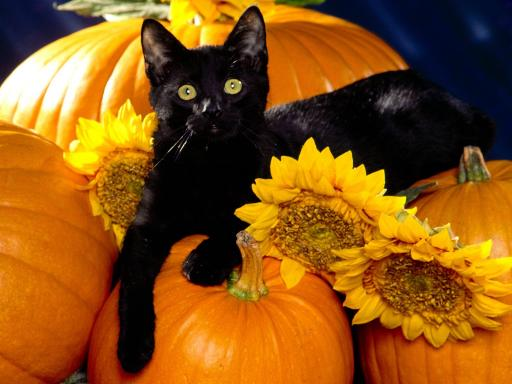
\includegraphics[scale=0.6]{SLEEP_APNEA/img/cat.png}
\caption{GUI aplikacji dla modułu SLEEP APNEA}
\label{fig:gui1}
\end{figure} 
Program został przetestowany na podstawie pięciu próbek pobranych z internetowej Bazy danych Physionet. Algorytm analizował dane próbkowane z częstotliwością 100Hz.
Na każdym z wykresów zostały przedstawione następujące elementy:
\begin{enumerate}
 \item \textbf {\color{blue}Znormalizowana amplituda sygnału}
 \item \textbf {\color{black}Maksymalna amplituda Hilberta}
 \item \textbf {\color{red}Okres bezdechu sennego}
 \item \textbf {\color{green}Okres bezdechu sennego}
 \item {Podsumowanie danych wyjściowych}
\end{enumerate}

Poniżej zamieszczono wykresy dla pięciu zestawów danych.
\newpage
\begin{figure}[H]
\centering
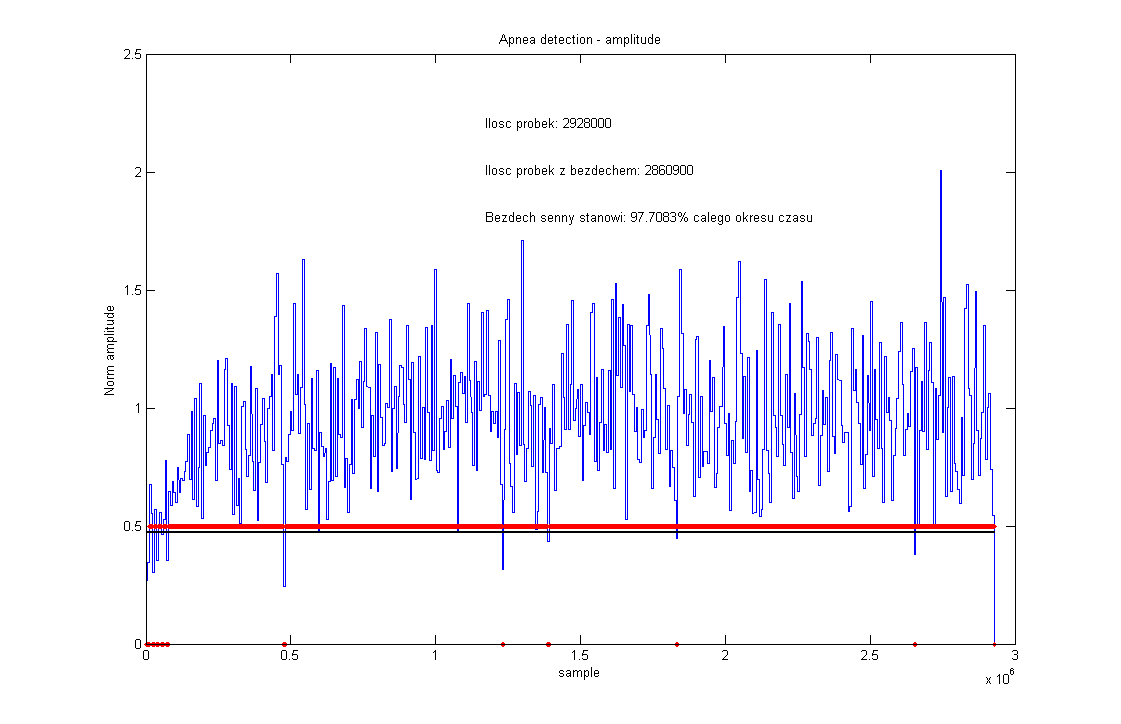
\includegraphics[scale=0.7, angle=90]{SLEEP_APNEA/img/apnea1.png}
\caption{Wykres końcowy programu dla danych a01}
\label{fig:apnea_1}
\end{figure} 
\newpage
\begin{figure}[H]
\centering
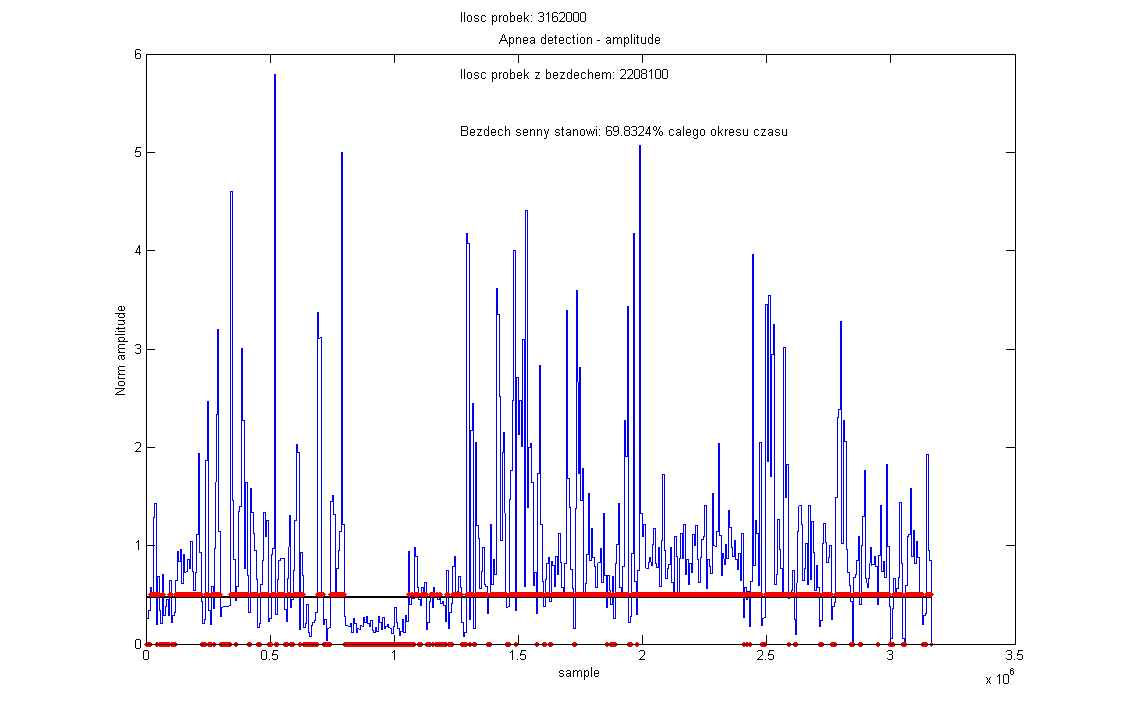
\includegraphics[scale=0.7, angle=90]{SLEEP_APNEA/img/apnea2.png}
\caption{Wykres końcowy programu dla danych a02}
\label{fig:apnea_2}
\end{figure}
 \newpage
\begin{figure}[H]
\centering
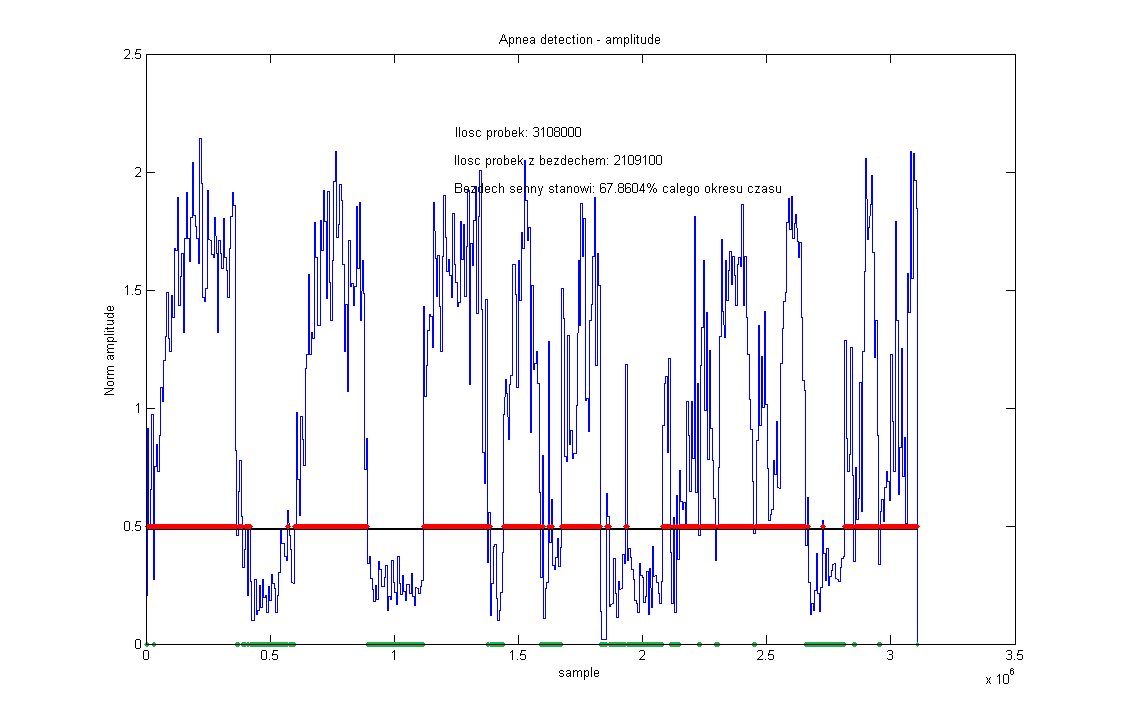
\includegraphics[scale=0.7, angle=90]{SLEEP_APNEA/img/apnea3.png}
\caption{Wykres końcowy programu dla danych a03}
\label{fig:apnea_3}
\end{figure} 
\newpage
\begin{figure}[H]
\centering
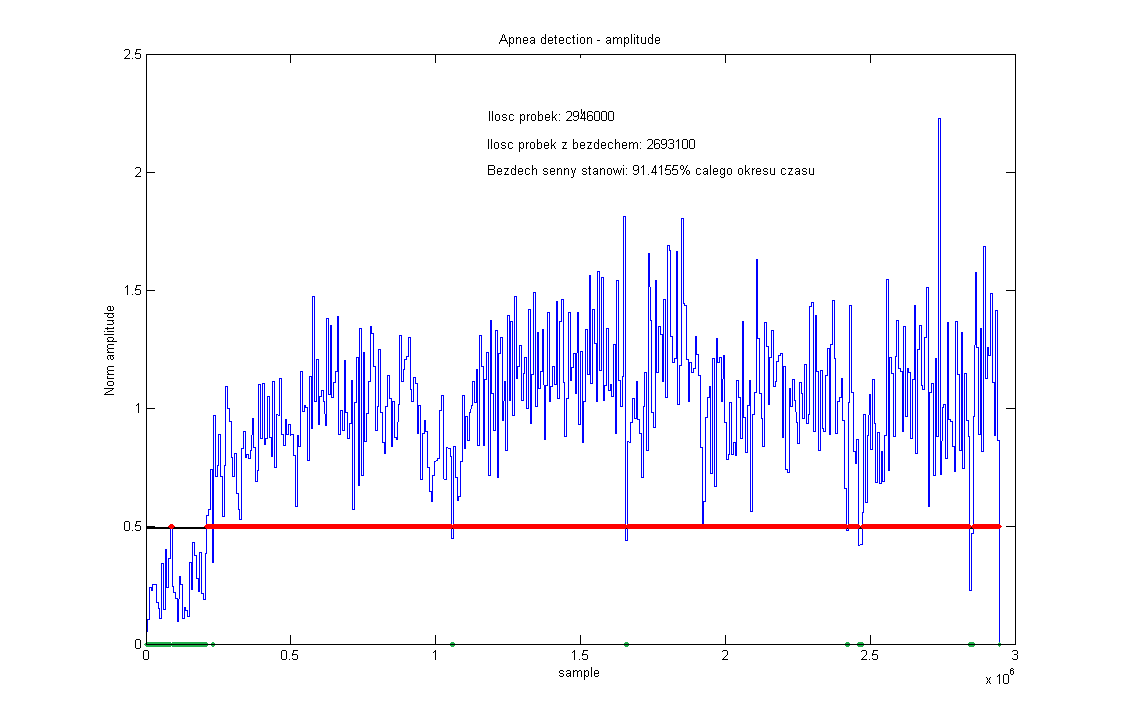
\includegraphics[scale=0.7, angle=90]{SLEEP_APNEA/img/apnea4.png}
\caption{Wykres końcowy programu dla danych a04}
\label{fig:apnea_4}
\end{figure}
\newpage
\begin{figure}[H]
\centering
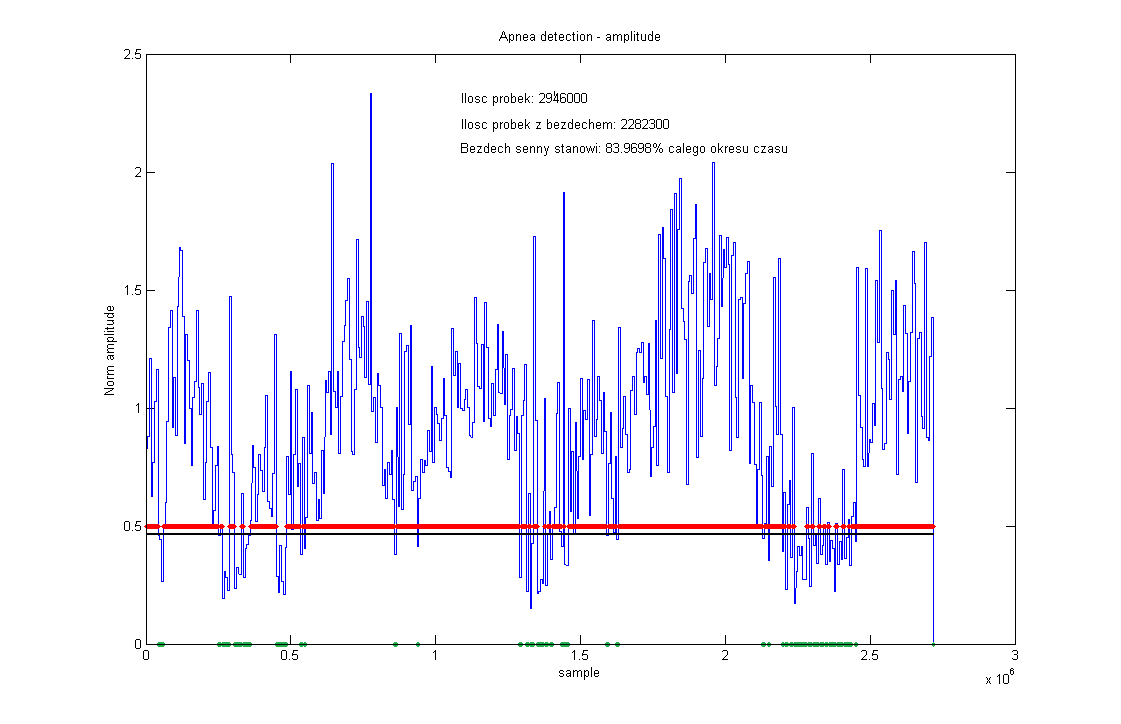
\includegraphics[scale=0.7, angle=90]{SLEEP_APNEA/img/apnea5.png}
\caption{Wykres końcowy programu dla danych a05}
\label{fig:apnea_5}
\end{figure} 
\newpage

Poniżej przedstawiono tabelę porównawczą dla omawianych wyżej przykładów. Są w niej zawarte wyniki badań specjalistów z Physionetu oraz wyniki sporządzonego algorytmu. 


\textbf{Współczynnik} opisywany w tabeli jest liczony następująco:
 \begin{equation}
 wsp =\frac{apnea}{ (end-begin)} 
 \end{equation}
gdzie: \newline
begin - numer pierwszej próbki rekordu \newline
end - numer ostatniej próbki rekordu \newline
apnea - ilość próbek w których wykryto bezdech senny \newline


\textbf{Ilość przedziałów} mówi o liczbie niezależnych odcinków czasu w całym sygnale, gdzie wykryto bezdech senny

\begin{table}[!ht]
  \centering
  \begin{tabular}{|c|c|c|c|c|}
    \hline
  &\multicolumn{2}{|c|}{Physionet}&\multicolumn{2}{|c|}{Algorytm} \\
    \hline
Dane&Współczynnik&Ilość przedzialów&Współczynnik&Ilość przedzialów \\
    \hline
    a01 & 95,69 & 3 & 97,71 & 10 \\
    a02 & 77,61 & 11 &  69,83 & 40 \\
    a03 & 45,37 & 11 &  67,86 & 28 \\
    a04 & 91,65 & 3 & 91,41 & 8 \\
    a05 & 57,62 & 15 & 83,97 & 36 \\
    \hline
  \end{tabular}
\caption{Tabela porównawcza dla danych pobranych z Physionetu oraz danych wyjściowych algorytmu }
\end{table}
Jak można zauważyć, zaimplementowany przez nas algorytm w większości przypadków identyfikuje bezdech senny w większej ilości próbek w porównaniu z badaniami pochodzącymi z bazy Physionetu. Taka zależność może byś spowodowana:
\begin{enumerate}
 \item Błędnym wykryciem R-pików
 \item Utratą części danych po etapach filtracji i przepróbkowania
 \item Wyliczaniem progowej wartości amplitudy na podstawie stałych współczynników
\end{enumerate}

W przypadku rekordu zdrowego człowieka algorytm wykrywa bezdech senny, ze względu na to, iż wartość progowa amplitudy jest ściśle powiązana z maksymalną i minimalną wartością amplitudy przetworzonego sygnału. Aby wyeliminować ten błąd należałoby wykrywać bezdech senny nie tylko na podstawie wyliczonej wartości progowej, ale także uwzględniając zewnętrze dane statystyczne, niezależne od badanego rekordu.
\subsection{Literatura}
[1] T. Penzel, J. McNames, A. Murray, P. de Chazal, G. Moody, and B. Raymond, “Systemantic compratition of different algorithms for apnoea detection based on electrocardiogram recordings,” Med. Biol. Eng. Comput.,vol. 40, no. 4, pp. 402–407, Jul. 2002.
\newline \newline
[2] Mendez M.O., Bianchi A.M., Matteucci M., Cerutti S., Penzel T.,” Sleep Apnea Screening by Autoregressive Models From a Single ECG Lead”, IEEE Transactions on Biomedical Engineering, Vol. 52, No. 12, 2009, pp. 2838-2850 
\newline \newline
[3] Isa S.M., Fanany M.I., Jatmiko W., Arymurthy A.M., “Sleep Apnea Detection from ECG Signal: Analysis on Optimal Features, Principal Components”, and Nonlinearity, International Conference on Bioinformatics and Biomedical Engineering, 2011, pp. 1-4 
\newline \newline
[4] J. E. Mietus, C. K. Peng, P. Ch. Ivanov, A. L. Goldberger, “Detection of Obstructive Sleep Apnea from Cardiac Interbeat Interval Time Series”, Beth Israel Deaconess Medical Center and Harvard Medical School, Poston, USA

\includegraphics[scale=1.4]{SLEEP_APNEA/img/blank.png}
\subsection{Diagram klas}
\begin{tikzpicture}
  \begin{class}[text width=15cm]{SleepApnea}{0,0}
    \attribute{dataFreq : int=samplingFreqency}
    \attribute{window : int = 41}
    \attribute{lfilt : int = 32}
    \attribute{windowMedian : int = 60}

    \operation{sleepApnea(samplingFreqency : const int)}
   \operation{sleepApnea plots(tabRpeaks : QVector<unsigned int>)}
    \operation{sleepApnea output(tabRpeaks : QVector<unsigned int>)}
    \operation{guiOutput(tabRpeaks : QVector<unsigned int>)}

    \operation{RRintervals(samplingFreqency : const int)}
    \operation{averangeFilter(tab RR : QVector<QVector<double> >)}
    \operation{resample(tabRRnew : QVector<QVector<double> >)}
    \operation{HpLpFilter(\&tabRes : QVector<QVector<double> >)}
    \operation{hilbert(tabRes : QVector<QVector<double> >,\&hAmp : QVector<QVector<double> >,\&hFreq : QVector<QVector<double> >)}
    \operation{freqAmpFilter(\&hAmp : QVector<QVector<double> >,\&hFreq : QVector<QVector<double> >)}
    \operation{medianFilter(\&hAmp : QVector<QVector<double> >,\&hFreq : QVector<QVector<double> >)}
    \operation{apneaDetection(tabAmp : QVector<QVector<double> >, tabFreq : QVector<QVector<double> >)}
  \end{class}
\end{tikzpicture}

\includegraphics[scale=0.8]{SLEEP_APNEA/img/blank.png}